
%\newcommand\invisiblesection[1]{%
%  \refstepcounter{section}%
%  \addcontentsline{toc}{section}{\protect\numberline{\thesection}#1}%
%  \sectionmark{#1}}
%enter chapter title here
%\invisiblesection{text you want to appear in pdf file}

\chapter{Research papers}

\newcommand\invisiblesection[1]{
  \refstepcounter{section}
  \addcontentsline{toc}{section}{\protect\numberline{\thesection}#1}%
  \sectionmark{#1}}
%\invisiblesection{My publications}


\section{Main contributions}
\printbibliography[heading=none,prefixnumbers=M,keyword=Main,resetnumbers]


\subsubsection*{My contributions to manuscripts:}
All manuscripts were written by me. Fl{\aa}tten proposed the \textit{Steady-state boundary conditions} (SSBC) used in papers~\cite{cp1,jp1}, and determined the flux-difference splitting coefficients of the LTS-HLL scheme~\cite[Proposition~2]{jp2}, and TVD conditions for the LTS-HLL scheme~\cite[Proposition~5]{jp2}. Fl{\aa}tten contributed to all articles by discussing the manuscripts and reported results. M\"{u}ller contributed to all articles by discussing the manuscripts and reported results.

\begin{journalpaper}{1~\cite{jp1}}
\invisiblesection{Journal paper 1~\cite{jp1}}

	{\bfseries Large Time Step Roe scheme for a common 1D two-fluid model} \\[1em]	
	Marin Prebeg, Tore Fl{\aa}tten and Bernhard M\"{u}ller                 \\[1em]	
	Applied Mathematical Modelling, Vol. 44, pp. 124--142, 2017. 
      
\end{journalpaper}

\clearpage
\shipout\null

%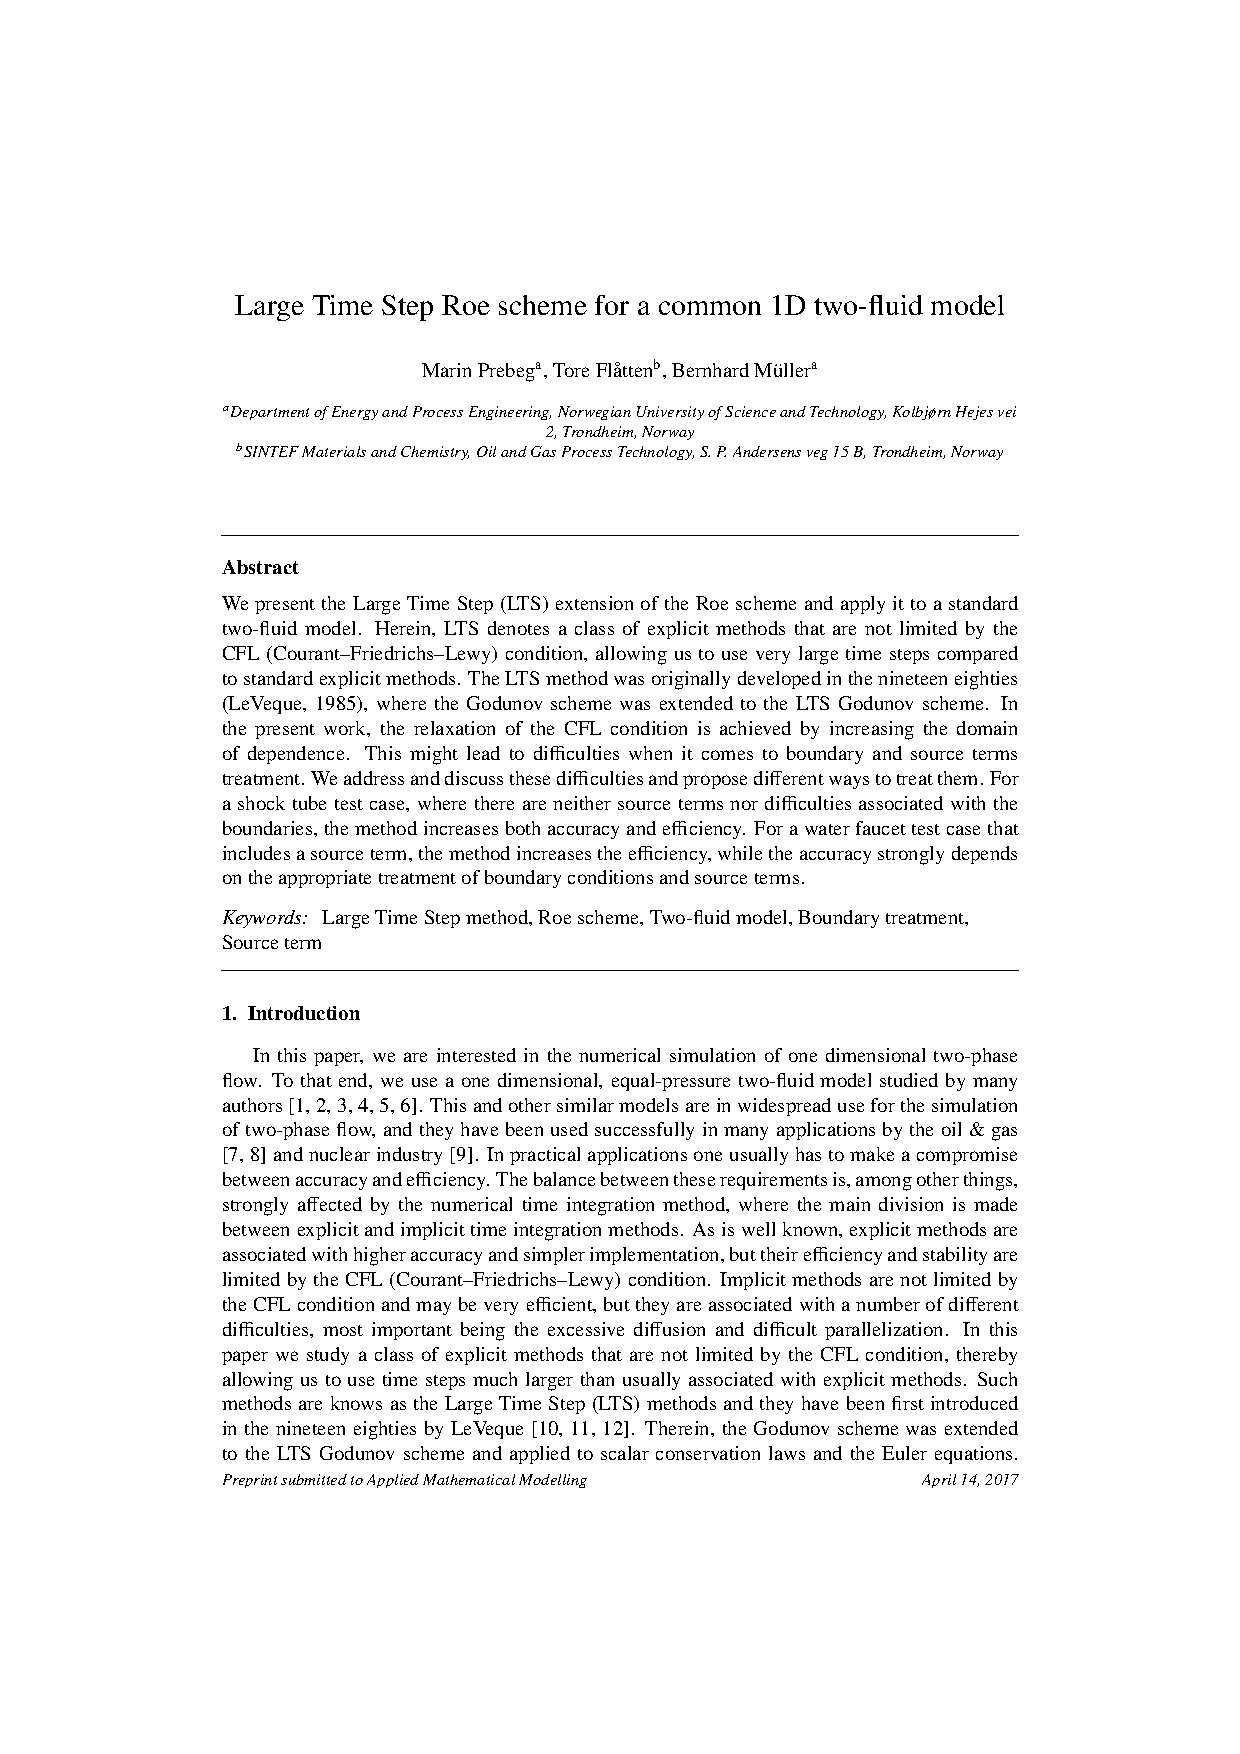
\includepdf[pages=-,pagecommand={\thispagestyle{empty}}]{Papers/AMM2017.pdf}

\clearpage
\shipout\null

\begin{conferencepaper}{1~\cite{cp1}}
\invisiblesection{Conference paper 1~\cite{cp1}}

	{\bfseries Boundary and source term treatment in the Large Time Step method for a common two-fluid model} \\[1em]	
	Marin Prebeg, Tore Fl{\aa}tten and Bernhard M\"{u}ller \\[1em]	
	In: Proceedings of the 11th International Conference on CFD in the Minerals and Process Industries. Melbourne, Australia, 2015.
  
\end{conferencepaper}

\clearpage
\shipout\null

%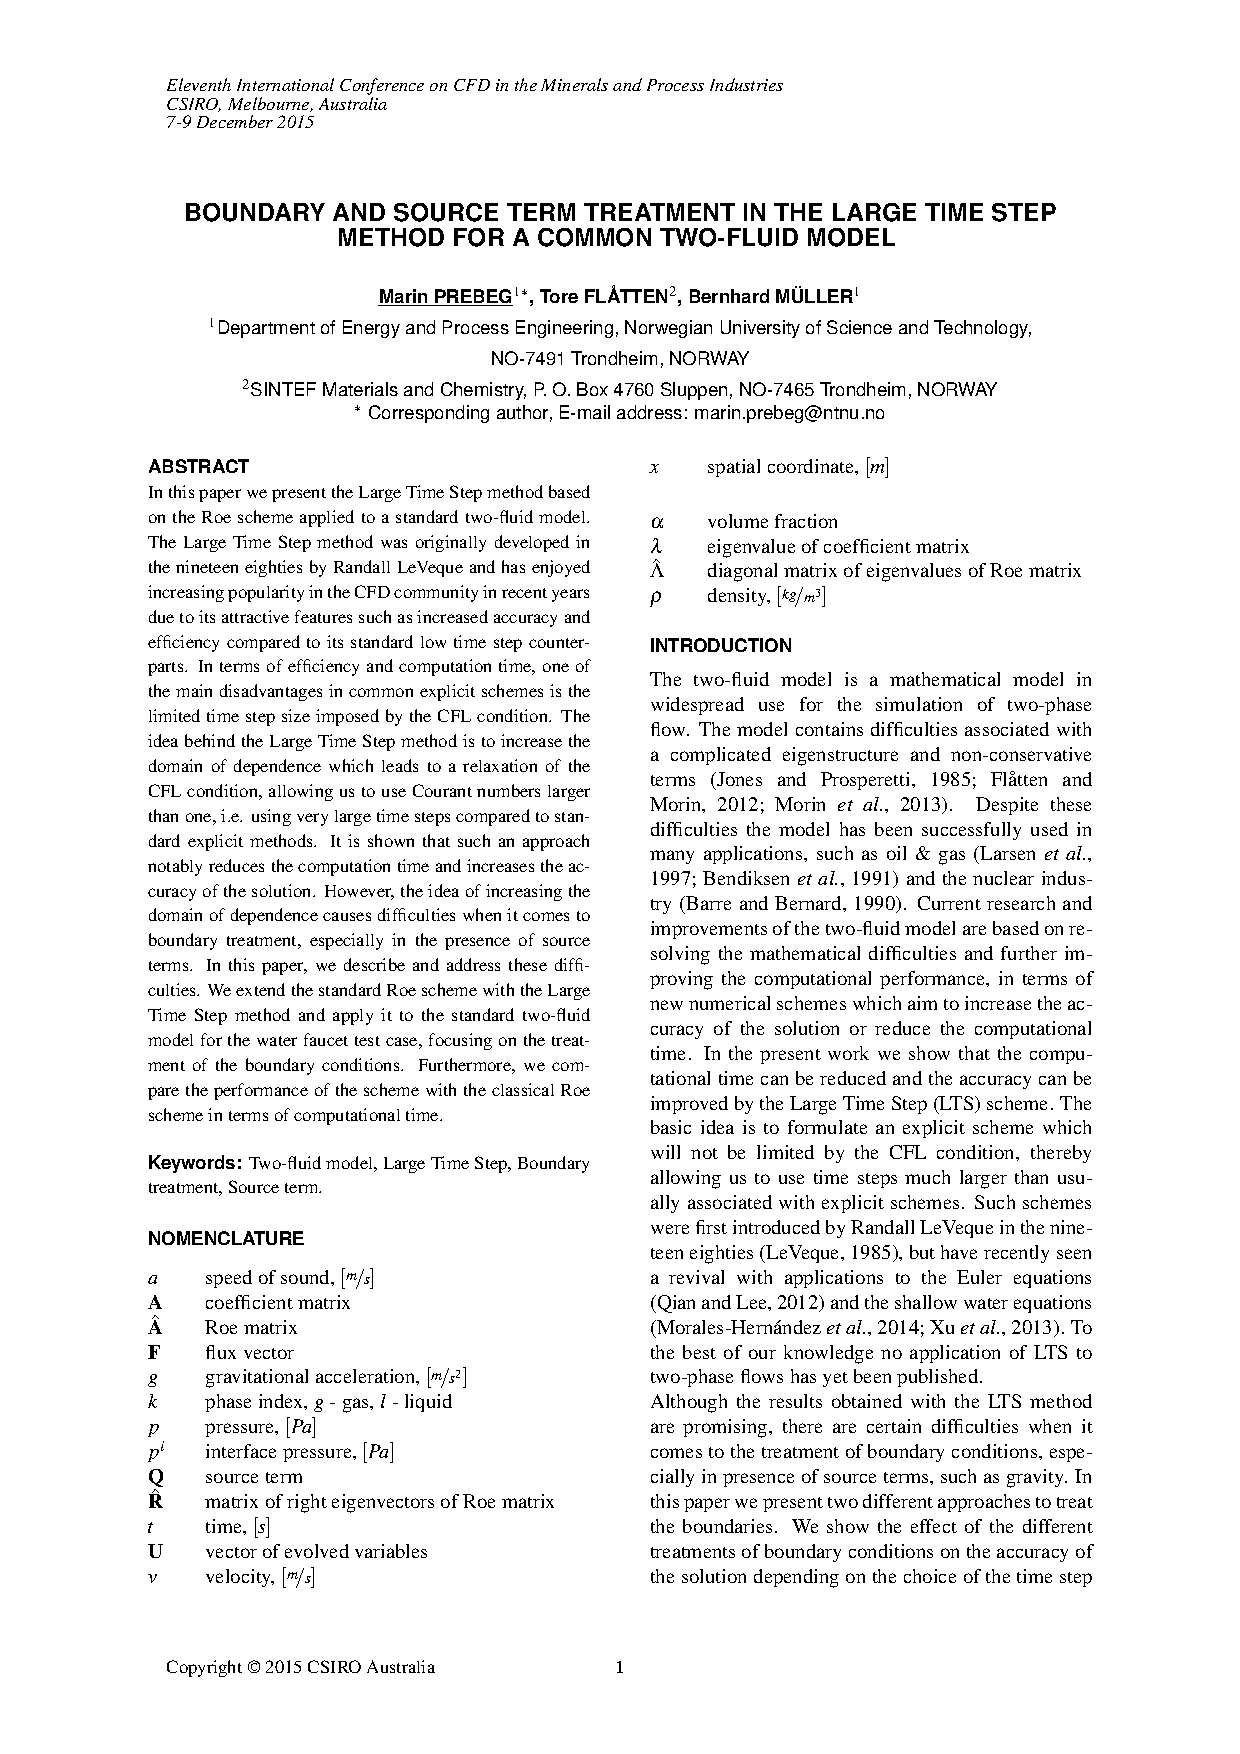
\includepdf[pages=-,pagecommand={\thispagestyle{empty}}]{Papers/CFD2015.pdf}

\clearpage
\shipout\null

\section{Additional contributions}
\printbibliography[heading=none,prefixnumbers=A,keyword=Additional,resetnumbers]


\subsubsection*{My contributions to manuscripts:}
All manuscripts were written by me. Fl{\aa}tten proposed the \textit{Steady-state boundary conditions} (SSBC) used in papers~\cite{cp1,jp1}, and determined the flux-difference splitting coefficients of the LTS-HLL scheme~\cite[Proposition~2]{jp2}, and TVD conditions for the LTS-HLL scheme~\cite[Proposition~5]{jp2}. Fl{\aa}tten contributed to all articles by discussing the manuscripts and reported results. M\"{u}ller contributed to all articles by discussing the manuscripts and reported results.

\begin{journalpaper}{1~\cite{jp1}}
	\invisiblesection{Journal paper 1~\cite{jp1}}
	
	{\bfseries Large Time Step Roe scheme for a common 1D two-fluid model} \\[1em]	
	Marin Prebeg, Tore Fl{\aa}tten and Bernhard M\"{u}ller                 \\[1em]	
	Applied Mathematical Modelling, Vol. 44, pp. 124--142, 2017. 
	
\end{journalpaper}

\section{Other works}
\printbibliography[heading=none,prefixnumbers=P,keyword=Other,resetnumbers]




